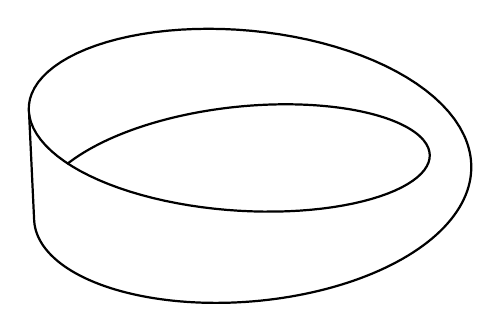
\begin{tikzpicture}[]
    \begin{axis}[
    hide axis,
    view={-15}{45},
    zmin=-0.2, zmax=0.2,
    samples=100,
    samples y=0,
    thick,
    draw=black,
    mark=none
    ]
        \addplot3
        [domain=0:135]
        (%
        {(1.0-0.1*cos(x/2))*cos(x)},
        {(1.0-0.1*cos(x/2))*sin(x)},
        {-0.1*sin(x/2)}
        );

        % \addplot3
        % [dashed,domain=135:170]
        % (%
        % {(1.0-0.1*cos(x/2))*cos(x)},
        % {(1.0-0.1*cos(x/2))*sin(x)},
        % {-0.1*sin(x/2)}
        % );

        \addplot3
        [domain=170:360]
        (%
        {(1.0-0.1*cos(x/2))*cos(x)},
        {(1.0-0.1*cos(x/2))*sin(x)},
        {-0.1*sin(x/2)}
        );

        \addplot3
        [domain=0:360]
        (%
        {(1.0+0.1*cos(x/2))*cos(x)},
        {(1.0+0.1*cos(x/2))*sin(x)},
        {0.1*sin(x/2)}
        );

        \addplot3
        []
        coordinates
        {
        ({(1.0+0.1*cos(166/2))*cos(166)},{(1.0+0.1*cos(166/2))*sin(166)},{0.1*sin(166/2)})
        ({(1.0-0.1*cos(170/2))*cos(170)},{(1.0-0.1*cos(170/2))*sin(170)},{-0.1*sin(170/2)})
        };
    \end{axis}
\end{tikzpicture}